\chapter{Hardware}
\section{Sensors}
\subsection{Lidar}

\subsection{Radar}
\subsubsection{Mount}
\subsection{IMU}
\section{Husky A200}
\subsection{Kinematics}
\section{Computers}


\chapter{Software}
\section{ROS system}
The work done in this project is a continuation and expansion of previous work \ref{Appdix:MAS513}. This previous work consisted of, among other things, configuring a Unmanned Ground Vehicle (UGV) along with sensors, in ROS2. There was therefore a desire to continue the work in this project in ROS2. The issue was that the pre-made package for the radar-modules was made for ROS1. The migration methods described on the official ROS2 documentation where attempted (described in \cite{ROSMigrationGuide}). Attempts where also made on using Amazon's tools for migrating ROS1 to ROS2 (described in \cite{ROSMigrationGuide}). Attempts on migrating the radar-package to ROS2 was ultimately abandoned. The perception system was implemented i ROS1, then the ROS1 bridge was utilised for communicating with the rest of the system which runs on ROS2.

\subsection{ROS1 system}
The ROS1 system is responsible for reading in data from a 3D-Lidar \ref and two radar-modules \ref, combining data and sending it on a format can be used for navigation purposes. The navigation system used in this project, and in \ref{Appdix:MAS513}, relays on the Laserscan message sent on the "/scan"-topic. The ROS1 system must provide the ROS2 system with the proper messages on the "/scan"-topic. Figure \ref{fig:rqt:ros1_noBridge} displays a rqt node-graph of the ROS1 system. The system is divided in to four main parts, which will be explained in the following parts.

Figure \ref{fig:simpleRos1Rqt} simplified presentation of the visualisation system running on ROS1. The nodes are represented by the red ovals, the green rectangles depicts the topics and the blue rectangles are used for groups, or common name spaces. All of the nodes, topics and "groups" that exists in a group share a common name space, like "$/namespace"$. For example, all the entities in the "$/radar0$" group begin their name with "$/radar0$". This naming convention serves two purposes, it allows , in a way, all the sensors to publish to the same topic name. For example, all of the sensors publishes to the "$/PointCloud$" topic, but no issues with similar names arises because they all use different naming prefixes. The second purpose is to allow the system to be viewed in a intuitive and structured way in the rqt node-graph.  

\begin{figure}[H]
\centering
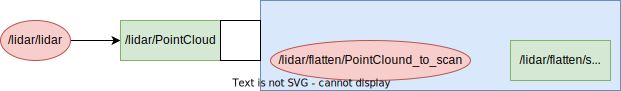
\includegraphics[scale=0.65]{Figures/draw.io/sipleRqtRos1.drawio.pdf}
  \caption{Simplifyed node-graph of ROS1 system}
  \label{fig:simpleRos1Rqt}
\end{figure}
%\subsection{Launch files}

The system is brought up with the help of launch files. One launch file (two in practice) is used to launch the entire, except the ROS1 bridge. The master launch file(s) are responsible for calling upon other "sublaunch" files. The sublaunch file system allows similar functionality to be re-used, similarly to how functions might be used in c or Python. All of the groups depicted in figure \ref{fig:simpleRos1Rqt} has a sublaunch file associated with it. The next parts will be use to explain the sublaunch files used by the main launch file(s). 

\subsubsection{}

The simplest way to initialise a ROS-node is to first start the roscore, then run the "rosrun" command in the Ubuntu terminal. Running a ROS-node can look something like the following example.  
\mint{css}{rosrun "package" "node-name" "argument-name":="value"}
However, This method becomes cumbersome once there is a need for running several nodes, with their own arguments. Each node would require their own terminal window, in addition to the roscore. The solution to this issue is launch files. Launch files makes it possible 

\subsection{Implementation}




\subsubsubsection{radar0 and radar1}




%\begin{figure}[H]
%\centering
%\includesvg[scale=0.14]{Figures/ros/ros1graph_noBridge.svg}
%  \caption{rqt node-graph of ROS1 system (see %\ref{Appdix:rqtROS1NB} for a bigger figure)}
%  \label{fig:rqt:ros1_noBridge}
%\end{figure}


\begin{table}[h!]
\centering
\begin{tabular}{c |c| c}
                &   Laptop              &   SBC and Laptop  \\
    \hline
    Ubuntu      &   18.04 (Bionic)      &   20.04 (Focal)   \\
    \hline
    ROS1        &   Melodic Morenia     &   Noetic Ninjemys \\  
    \hline
    ROS2        &   Eloquent Elusor     &   Galactic Geochelone\\
\end{tabular}
\caption{Table to test captions and labels.}
\label{table:1}
\end{table}